\documentclass[11pt]{article}

\usepackage[review]{acl}

\usepackage{times}
\usepackage{latexsym}
\usepackage[T1]{fontenc}
\usepackage[utf8]{inputenc}
\usepackage{microtype}
\usepackage{inconsolata}
\usepackage{graphicx}
\usepackage{booktabs}
\usepackage{amsmath}
\usepackage{tcolorbox}

\title{ENSAR at AraSeg Shared Task 2026: \\ An Ensemble of Encoders With Agentic Error Refinement}

\author{Noor Emam \\
  The American University in Cairo \\
  \texttt{noortaytoy1@aucegypt.edu} \\\And
  Omar Saqr \\
  The American University in Cairo \\
  \texttt{TODO@aucegypt.edu} \\\AND
  Mostafa Gafaar \\
  The American University in Cairo \\
  \texttt{TODO@aucegypt.edu} \\\And
  Aly El-aswad \\
  The American University in Cairo \\
  \texttt{TODO@aucegypt.edu} \\}

\begin{document}
\maketitle

\begin{abstract}
Half of our encoder ensemble's errors are sites where all five models agree with each other and disagree with the annotator, so no amount of ensembling or recalibration can fix them. We argue the next step in sentence segmentation is not bigger encoders but models that reason about why they were wrong. On top of the ensemble, which labels each token as sentence-final or not, we train two reasoning juries the way RLHF trains a policy, with the gradient step replaced by writing: each jury segments a training document, is shown every error beside the gold answer, and writes the rule it should have followed into its own instruction file. At inference the juries argue each document, and only the edits both endorse are applied. The juries add an average of 2.8 F1 across the four tracks, close to five points where punctuation is absent and under one where it is present, and the full system ranked first on three of the four tracks.
\end{abstract}

\section{Introduction}

Sentence segmentation is the first step of most NLP pipelines, and it is treated as
solved because in edited, well punctuated text the boundary signal sits on the
punctuation itself. \citet{read2012sentence} argued that this framing is too narrow:
systems that only disambiguate terminal marks yield overly optimistic estimates, and
performance collapses on text whose genre or structure departs from newswire. Arabic
realizes that warning in full. Punctuation is ambiguous and inconsistently used, many
texts carry no reliable boundary markers at all
\citep{elkholy2026arabicsentencesegmentationgenres}, and the conjunction \textit{wa}
begins sentences as readily as it joins clauses inside one. This shared task
\citep{elkholy-etal-2026-araseg-shared-task} makes the hard case explicit: its corpus
spans eight genres, and two of its four tracks remove punctuation from the input
entirely, so a boundary has no surface mark at all.

The literature answers missing punctuation in two ways. One line restores the punctuation
first and segments afterwards \citep{tilk2016bidirectional}. The stronger line classifies
boundaries directly without it: WtP trains a punctuation-agnostic character classifier on
newline supervision across 85 languages \citep{minixhofer2023wheres}, and SaT hardens it
with a pretraining scheme built for missing punctuation, beating every baseline including
strong LLMs on poorly formatted text \citep{frohmann2024segment}; for punctuated input,
ersatz classifies candidate punctuation contexts across 23 languages
\citep{wicks2021unified}. Every one of these systems is a classifier: it assigns each
position a boundary probability from local evidence, and when it is wrong it cannot say
why, nor which sentence convention the document follows. Cross-genre generalization is
precisely what the task corpus reports as still hard
\citep{elkholy2026arabicsentencesegmentationgenres}.

Our error analysis says the same thing from inside (Appendix \ref{sec:erroranalysis}): half
the errors of our five voter encoder ensemble are sites where every voter agrees and
every voter is wrong, at a median ensemble probability of 0.86. These are confident,
shared errors; no threshold, calibration, or additional voter removes them, because what
is missing is not a sharper probability but the annotation convention of the document at
hand. We therefore make the second stage reason: juries (Claude Opus 5 at maximum
reasoning effort) learn each genre's convention from their own graded mistakes on the
training split and edit the ensemble's proposals, adding an average of 2.8 $F_1$ across
the four tracks and ranking first on three of them.

\paragraph{Our approach.} We learn each document's annotation convention explicitly,
using the shape of RLHF
\citep{christiano2017deep, ouyang2022training} with the gradient step replaced. A language
model, which we call a jury, attempts a training document. The human annotations serve as
the reward: the attempt is scored, and every false cut and missed boundary is returned to
the jury in context beside the gold. The jury then works out for itself why it went wrong
at each site, revisiting the reasoning it used there, and writes the rule it should have
followed into its own instruction file. That file is the policy. The document is then
forgotten. Since nothing else survives between batches, whatever the jury learns has to be
written down to survive at all, which forces the policy to be explicit and leaves it open
to inspection.

\paragraph{Contributions.}
\begin{enumerate}
\itemsep0em
\item A training loop in which the thing being improved is a written set of instructions,
and the feedback is the annotator's answer at every token rather than a single score or the
model's own opinion of its work (Section \ref{sec:loop}).
\item An adjudication step in which two policies trained on disjoint halves of the corpus
argue each document and only the edits both endorse are applied (Section \ref{sec:adj}).
\item A controlled measurement of what the reasoning layer contributes over a strong
neural baseline, with edit directions that reverse between tracks
(Section \ref{sec:results}).
\item The learned instruction files themselves, which state when a sentence ends in each
kind of text along with the errors that taught it (Section \ref{sec:inside}).
\end{enumerate}

\section{Related Work}

RLHF optimises a policy against human preference through a reward model and a gradient
update \citep{christiano2017deep, ouyang2022training}. Our loop keeps the reward and the
policy improvement and discards the gradient: the parameters never change and the policy
lives in text.

Reflexion \citep{shinn2023reflexion} reinforces an agent verbally from task outcomes, and
Self-Refine \citep{madaan2023selfrefine} iterates a model against its own critique. Our
signal is neither: it is the annotator's label at the exact token the jury got wrong,
which matters because our errors are confident ones, and a system critiquing itself would
ratify them.

OPRO \citep{yang2024optimizers} optimises a prompt from scores on previous candidates, and
TextGrad \citep{yuksekgonul2024textgrad} propagates textual critique through a compound
system. Both optimise text; we differ in the supervision, which is dense and localised
rather than aggregate, and in the artifact, a persistent domain theory rather than a tuned
instruction string.

\section{Task and Data}

Every whitespace token must be labelled as sentence-final or not. Four tracks cross two
conditions: punctuation present or removed, and paragraph structure retained or removed.
In the paragraph-aware tracks (PA, NoPnx-PA) paragraph breaks survive as newline tokens,
which are informative, since the token before a paragraph break always ends a sentence and
a newline token never carries a boundary. In the no-paragraph tracks (NP, NoPnx-NP) that
signal is gone. The final token of a document always ends a sentence. We entered all four
tracks in the closed and open settings; the organizers ruled that post-editing an
encoder system with a pretrained language model is permitted in both, and that the
development and test splits may be used for model selection but never as training data,
which is how we used them.

Each track provides 174 training documents, 222 development documents and 262 test
documents, with a blind evaluation set of 212 documents for the no-paragraph tracks and
100 for the paragraph-aware tracks. Boundaries are sparse: 8.3\% to 10.4\% of tokens
depending on track.

\section{System}

\subsection{Encoder ensemble}

We fine-tune four pretrained encoders: AraBERTv0.2-base, AraBERTv0.2-large,
Arabic-BERT-large and XLM-RoBERTa-large. AraBERTv0.2-large is fine-tuned twice, once with
FGM adversarial training at $\epsilon = 1.0$ and once with an auxiliary supervised
contrastive loss at weight 0.1, giving five voters. Each is trained for 10 epochs on
overlapping windows of 180 words with stride 90, with cross-entropy in which the boundary
class is weighted by the training negative-to-positive ratio capped at 8. Probabilities
are averaged across voters and across overlapping windows.

Rather than thresholding, we decode with a semi-Markov dynamic program that trades
boundary probability against the plausibility of the resulting segment lengths under a
distribution fitted on the training split:
\begin{equation}
\hat{B} = \arg\max_{B} \sum_{i \in B} \log p_i + \lambda \sum_{s \in \mathrm{seg}(B)} \mathcal{L}(|s|) - \beta |B|
\end{equation}
with $\lambda = 0.4$ and $\beta = 0.75$. The length prior is refitted on the first pass
output, blended with the corpus prior at weight 0.7, and the document is decoded again.
Structurally certain boundaries are forced. All fine-tuning uses the training split only;
the development split is used for checkpoint selection and for these hyperparameters.

\subsection{Learning a policy from graded errors}
\label{sec:loop}

A jury is defined entirely by one text file, which it writes itself. Training proceeds in
batches of five training documents:

\begin{enumerate}
\itemsep0em
\item \textbf{Attempt.} The jury reads its current policy, then segments each document
from scratch, one at a time, recording each boundary as a token index with the token
itself.
\item \textbf{Reward.} The attempt is scored against the training gold. Boundaries match
within a tolerance of two tokens against an identical surface form, so indexing drift is
not scored as a segmentation error.
\item \textbf{Diagnosis.} Every wrong cut and every missed boundary is handed back to the
jury in context, with its own answer and the annotator's answer shown side by side at the
same place in the text.
\item \textbf{Policy update.} The jury diagnoses the rule behind each error and writes it
into its policy file, with its own failure as the worked example. Entries that later
evidence contradicts are revised in place.
\item \textbf{Reset.} The documents are discarded. The next batch begins with the updated
policy and no other memory.
\end{enumerate}

Two juries are trained this way on disjoint halves of the corpus, 87 documents each, so
that their policies are genuinely different. For NoPnx-PA the resulting files are 1{,}398
and 2{,}098 lines.

The doctrines record this process in the juries' own words. Superseded rules are struck
through and kept for the trail, every revision names the graded errors that forced it,
and Appendix \ref{sec:learning} reproduces two full revision arcs verbatim: a default
learned in batch 1, inverted by batch 2's errors, and replaced in batch 13 by a synthesis
that neither earlier default contains.

Figure \ref{fig:update} shows a real update: a hypothesis, contrary graded evidence, and
an explicit revision that survives into every later document.

\begin{figure}[t]
\scriptsize
\begin{tcolorbox}[colback=white, boxrule=0.4pt, left=3pt, right=3pt, top=3pt, bottom=3pt]
\textbf{LAW 5, batch 2 (abridged, verbatim).}
``Off-by-one-clause remains a real, separate failure mode. In batch 2 nearly every one of
my 16 misses was paired with a false cut 1--2 clauses away: I had the right idea and the
wrong site. \textbf{REVISION to the batch-1 tactic.} Batch 1 said the annotators cut at the
\emph{first} available \textit{wa}/\textit{fa} in a run, not the second. Batch 2 shows the
opposite as often as not, so the first-joint heuristic is retired.''
\end{tcolorbox}
\caption{A policy update written by a jury after its second graded batch, retiring a rule
it had induced from the first. Each entry cites the document and token offsets of the
errors that forced the change.}
\label{fig:update}
\end{figure}

\subsection{Adjudication: only edits both juries endorse}
\label{sec:adj}

At inference the two juries consider one document at a time, presented with the ensemble
boundaries already marked and described as an unreliable draft they may consult but must
not trust. Each states its reading from its own policy, and they argue every site on which
they differ, with a rule earned from a graded error in the genre at hand outranking an
unsupported intuition. Only edits that both juries endorse are applied; unresolved
disagreements leave the ensemble boundary in place, and leaving a document unchanged is an
admissible verdict. Edits are recorded as token positions with surface forms and applied
under the same two-token tolerance and the same structural constraints used in training.

The value of separate training shows in the transcripts: on one scripture document, one
jury argued an edit from verse structure and the other from rhyme, and they endorsed the
same edit by different routes. Agreement of that kind is evidence; agreement between two
copies of one policy would not be.

Training and inference deliberately differ in one respect: in training the jury segments
from scratch and sees no draft, at inference it edits the ensemble's draft. Training from
scratch is what forces the policy to be complete, since a jury that only ever corrected
a draft could learn to defer to it; the object learned is a statement of where sentences
end in each kind of text, which applies equally to writing boundaries and to judging
them. Whether it transfers is an empirical question, and Table \ref{tab:ablation} is the
answer: the from-scratch policies improve the draft on every track.

\section{Results}
\label{sec:results}

\subsection{Official results}

Our system ranked first on Pnx-PA, Pnx-NP and NoPnx-NP in both the closed and open
settings, with blind $F_1$ of 95.30, 92.0 and 89.1, and scored 90.0 on NoPnx-PA, where it
did not place first. The NoPnx-PA juries had to be rebuilt from scratch in the final
hours before the deadline and were trained on 60 of the 174 training documents; the
retrained pair in Table \ref{tab:ablation} is the same system with that training
completed.

\subsection{What the reasoning layer contributes}

The leaderboard cannot separate the two stages, since only the combined system was
submitted. We therefore compare arms on the released test split: identical documents,
identical gold, and the only difference being whether the jury edits are applied. Because
the juries edit the ensemble output rather than replacing it, the difference isolates the
reasoning layer.

\begin{table}[t]
\centering
\scriptsize
\setlength{\tabcolsep}{2.5pt}
\begin{tabular}{lcccc}
\toprule
 & \textbf{NoPnx-NP} & \textbf{NoPnx-PA} & \textbf{NP} & \textbf{PA} \\
\midrule
Ensemble        & 84.64 & 87.05 & 92.83 & 94.56 \\
+ juries        & \textbf{89.49} & \textbf{92.28} & \textbf{93.61} & \textbf{94.92} \\
$\Delta$        & +4.85 & +5.23 & +0.77 & +0.36 \\
\midrule
Docs $+/-/=$    & 186/28/48 & 164/35/63 & 80/38/144 & 58/44/160 \\
Bounds $+/-$    & 923/417 & 554/702 & 192/203 & 141/113 \\
\midrule
Paired $t$, $p$ & $10^{-13}$ & $10^{-13}$ & $10^{-4}$ & $.024$ \\
95\% CI         & [3.6, 6.1] & [3.9, 6.6] & [0.4, 1.2] & [.05, .67] \\
\bottomrule
\end{tabular}
\caption{Ablation on the 262-document test split, macro $F_1$: documents
improved/degraded/unchanged and boundaries added/removed. The baseline row is purely
neural: the ensemble's blind predictions reproduce exactly from the cached voter
probabilities, so no rule-based post-processing sits between the encoders and the juries.
The submitted systems are the ensemble plus the juries.}
\label{tab:ablation}
\end{table}

Two properties of this comparison should be stated. The NP, PA and NoPnx-NP juries are the
ones used for our submission, while the NoPnx-PA juries were retrained on the full
training corpus after the deadline, since the submitted pair had been trained on part of
it under time pressure; that row is therefore an unofficial post-deadline result. The
ablation baseline is a thresholded average rather than the length-aware decode used for
submission and on the NoPnx tracks scores about half a point lower on test. Neither
affects the sign or the significance.

\subsection{A policy, not a threshold}

The most diagnostic numbers in Table \ref{tab:ablation} are the edit directions. On
NoPnx-NP the juries add 923 boundaries and remove 417. On NoPnx-PA they add 554 and remove
702. The ensemble under-segments when punctuation and paragraph structure are both absent
and over-segments when paragraph tokens are present, and the juries correct each. No
change of threshold, temperature or decoding penalty produces opposite corrections on two
tracks from one system. The layer is conditioning on what the document is, which is what a
policy does and what a confidence adjustment cannot.

The two punctuated tracks complete the picture. There the juries make a fraction of the
edits, 395 on NP and 254 on PA against 1{,}340 and 1{,}256 on the NoPnx tracks, leave more
than half of all documents untouched, and the gain falls from about five points to under
one, still positive on both tracks. The layer contributes most exactly where the surface
signal is weakest and stands down where punctuation already marks the boundaries: the
learned policy substitutes for the missing punctuation rather than duplicating it.

Degradations concentrate in documents where both juries shared a reading the annotators did
not. Requiring both juries to agree filters out disagreement, not shared error, which
bounds what this design can fix.

\subsection{What the learned policies contain}
\label{sec:inside}

The policies are plain text, so we can read what the system learned.

The first rule one jury applies to any new document is to count. Before marking a single
boundary it measures how many words fall between paragraph breaks. If the lines are short,
the line is the sentence, and it should cut at the line breaks and almost nowhere else. If
the lines are long, sentences end inside them and it must look. The jury wrote this rule
after scoring 33.3 on a multiple choice exam bank, where it had applied rules learned from
prose to a document that contains no prose.

A second rule is about how long a sentence is expected to be, and it turns out to depend on
what the reader is holding. The same jury keeps separate expectations for a children's
picture book (about 10.6 words per sentence), a children's magazine feature (about 14.3), a
classical folk narrative (about 11) and a translated monograph (about 20.3). It separated
them because treating them alike had cost it points.

The third is the correction in Figure \ref{fig:update}: a rule induced from one batch,
refuted by the next, and retired in writing, with the diagnosis that its misses sat one or
two clauses from a false cut nearby, the right instinct at the wrong site.

Both juries reached the same conclusion near the end of training, independently: their worst
errors came from carrying the sentence length of one document into the next because the two
looked superficially alike. Both responded by making the question ``what kind of text is
this'' an explicit first step. None of this is expressible by our encoders, and none of it
was written by us.

\section{Conclusion}

We described a two-stage system for Arabic sentence segmentation in which an encoder
ensemble is refined by a reasoning layer whose policy is learned from graded errors on the
training data and stored as text rather than weights. The system ranked first on three of
the four shared task tracks. A controlled ablation shows the reasoning layer is worth close to five
$F_1$ points on the two no-punctuation tracks, a smaller but reliable gain when punctuation
is present, and that it corrects opposite biases under different input conditions. We take
this as evidence that a meaningful part of the remaining headroom in Arabic segmentation
is not probabilistic but definitional: it lies in genre-specific conventions that can be
recovered by reasoning over graded errors and stated in language, but not by estimating
better probabilities over the same features.

\section*{Limitations}

The reasoning layer is expensive. Adjudicating one document costs on the order of tens of
thousands of tokens, several orders of magnitude more than an encoder forward pass, and the
cost grows with document length. The method suits settings where segmentation quality
outweighs throughput.

The juries are a proprietary model (Claude Opus 5) accessed through an API, and decoding is
not deterministic, so exact reproduction depends on that model version remaining available.
We release the learned policies and the prompts, so the stage can be inspected and audited
even where it cannot be re-derived bit for bit.

When both juries share a wrong reading, nothing in the design catches it; every one of our
degraded documents is of that kind. All results are from one corpus in one language.

\section*{Acknowledgments}

TODO.

\bibliography{custom}

\appendix

\section{Reproducibility}
\label{sec:appendix}

\paragraph{Voter recipes.} All five voters: 10 epochs, windows of 180 words with stride 90,
maximum sequence length 512, cross-entropy with the boundary class weighted by
$\min(\mathrm{neg}/\mathrm{pos}, 8)$, which evaluates to 8.00 on every track. Defaults are
learning rate $5{\times}10^{-5}$ and batch size 16. Differences: \texttt{imp\_fgm} is
AraBERTv0.2-large with FGM $\epsilon = 1.0$; \texttt{boost\_supcon01} is AraBERTv0.2-large
with supervised contrastive weight 0.1; \texttt{xlmr-2e5} is XLM-RoBERTa-large at learning
rate $2{\times}10^{-5}$ and batch size 4; \texttt{nat\_arabertv02\_base} is
AraBERTv0.2-base and \texttt{nat\_asafaya\_large} is Arabic-BERT-large, both at defaults.
Checkpoints are selected on the development split. For Pnx-PA a tuned three-voter subset
with $\beta = 0.6$ was used at submission.

\paragraph{Corpus statistics.} Training boundary rate is 0.104 (NoPnx-NP), 0.101
(NoPnx-PA), 0.086 (NP) and 0.083 (PA), over 98{,}457, 101{,}784, 124{,}444 and 128{,}173
tokens respectively.

\paragraph{Metric.} We report macro $F_1$, the per-document mean. Token-pooled micro values
are higher because errors concentrate in long documents: on test the ensemble scores 86.23
micro against 84.64 macro on NoPnx-NP, 89.30 against 87.05 on NoPnx-PA, 93.76 against
92.83 on NP, and 95.76 against 94.56 on PA.

\paragraph{Jury prompts.} The two prompts below are the exact texts run for the NoPnx-PA
juries (Claude Opus 5, maximum reasoning effort), with local file paths and the per-jury
document lists replaced by placeholders in angle brackets. The other tracks use the same
prompts with the FORMAT paragraph swapped for that track's input convention.

\subparagraph{Training prompt (one per jury, $j \in \{0, 1\}$).}
\begin{tcolorbox}[colback=white, boxrule=0.4pt, left=3pt, right=3pt, top=3pt, bottom=3pt]
\scriptsize\ttfamily\raggedright
You are Jury <j>, a brand-new Arabic sentence-segmentation judge. You start with zero
knowledge of this corpus's conventions, everything you will ever know comes from your own
graded attempts on TRAINING documents. Work in <repo>.\\
The ONLY files you may touch: the practice documents listed below, your own answer files,
the grader's mistakes file named below, and your own doctrine file <doctrine\_j>.md.
Touching ANY other file voids the training, answer keys exist elsewhere in this
repository.\\
FORMAT: Punctuation REMOVED; paragraph structure KEPT as literal <NL> tokens (each <NL>
has its own index). The \P{} on the token immediately before every <NL> and on the final
token is ALWAYS correct and must never be removed; an <NL> token itself NEVER carries a
boundary. Everything inside paragraphs is yours to judge. <i> = index anchor, not part of
the text.\\
YOUR DOCUMENTS, in batches of five, in this order: <87 document ids>\\
PER BATCH:\\
1. SEGMENT strictly one document at a time from <train\_docs>/<doc\_id>.json. No limit on
your reasoning, first work out what the text IS (genre, register, structure) and what its
natural sentence unit is, then walk it and argue every uncertain site in writing. Write
your answer to <ans\_j>/<doc\_id>.json as \{"doc\_id":"...","identity":"what this text
is","law":"its sentence law as you read it","reasoning":"your argument at the hard
sites","boundaries":[\{"i":<index of the LAST token of a sentence>,"w":"<that token
copied from the text>","c":"hi|med|lo"\}]\} the moment it is done, before opening the
next document. Use ONLY properly escaped JSON, no raw newline characters inside strings.\\
2. GRADE: run python grade4.py --track nopa --juror <j> --only <the five ids
comma-separated> and read <mistakes\_j>.txt in full.\\
3. LEARN: for every FALSE CUT and every MISSED, find the RULE behind it, what do these
annotators actually do, and write it into your doctrine file in your own words, filed by
text type, with your own error as the example. When a new correction contradicts an
earlier entry, fix the earlier entry and say so. The doctrine is cumulative, never delete
knowledge.\\
4. Take your updated doctrine into the next batch.\\
If you hit a usage limit or crash, everything is already saved; on restart, skip
documents whose answer file exists. When all batches are graded and absorbed, return your
per-batch mean F1 and 4 sentences on your doctrine's core laws. No web. No PowerShell
except the grader command given above.
\end{tcolorbox}

\subparagraph{Adjudication prompt (one per sitting of four documents).}
\begin{tcolorbox}[colback=white, boxrule=0.4pt, left=3pt, right=3pt, top=3pt, bottom=3pt]
\scriptsize\ttfamily\raggedright
This is exam sitting <n> of <total>. Two TRAINED juries sit together: Jury 0 and Jury 1.
Each trained separately on this annotation team's training documents and wrote its own
doctrine from its own graded mistakes. You hold both: when Jury 0 speaks, reason strictly
from doctrine 0; when Jury 1 speaks, strictly from doctrine 1. They are colleagues with
different training histories, not one voice twice.\\
FIRST read both doctrines ONCE: Jury 0: <doctrine\_0> Jury 1: <doctrine\_1>\\
FORMAT: Punctuation REMOVED and paragraph structure KEPT as literal <NL> tokens. The \P{}
on the token immediately before every <NL>, and on the final token, is ALWAYS correct and
must never be removed; an <NL> token itself NEVER carries a boundary. <i> = index anchor,
not part of the text.\\
YOUR 4 DOCUMENTS, one file each, STRICTLY ONE AT A TIME (finish and record one before
opening the next): <four packet paths>\\
Each document arrives with an automatic system's boundary marks (\P) already drawn in.
Treat them as an UNRELIABLE CHEAT SHEET: allowed to consult, never to trust, it makes both
kinds of errors. A document whose marks already satisfy its law is FINISHED; unchanged is
a common and correct verdict.\\
PER DOCUMENT, no limit on your reasoning depth:\\
1. Jury 0 gives its full stance from doctrine 0, what the text is, which register it
belongs to, its sentence law, and every place the draft marks are wrong, argued from the
text.\\
2. Jury 1 gives its own independent stance from doctrine 1, site by site.\\
3. They ARGUE every disagreement. Concede when the colleague's reading matches the
annotators' policy better; rebut precisely when it does not. Where a doctrine carries a
law earned from a graded mistake in THIS register, that law outranks instinct.\\
4. RECORD: only changes BOTH juries endorse survive. Unresolved means the draft stands.
Write \{"doc\_id":"...","add":[\{"i":<index>,"w":"<token>"\}],"remove":[\{"i":<index>,
"w":"<token>"\}],"argued":"<one line per argued site>"\} to <exam\_out>/<doc\_id>.json
IMMEDIATELY on finishing that document. add = token positions that end a sentence but
carry no \P; remove = positions carrying \P{} that do not end a sentence; copy w from the
text at the moment you decide. Never add or remove on an <NL> token; never remove a \P{}
that sits immediately before an <NL> or on the final token.\\
RESUME: if <exam\_out>/<doc\_id>.json already exists, skip that document.\\
When all are recorded return \{"done": <count>, "note": ""\}. No web, no PowerShell.
Touch NOTHING beyond the two doctrine files, your listed documents, and your own output
files, answer keys for this corpus exist elsewhere in this repository and opening
anything else voids the evaluation.
\end{tcolorbox}

\section{Error analysis}
\label{sec:erroranalysis}

All numbers in this section are recomputed from the cached voter probabilities and the
released gold by our verification script. The setup is the NoPnx-NP track with each voter
and the ensemble mean thresholded at 0.5.

On the development split the ensemble makes 3{,}749 errors. 1{,}811 of them (48.3\%) are
sites where all five voters are on the wrong side of the threshold, the situation the
abstract describes: the models agree with each other and disagree with the annotator. At
the remaining sites the voters split, but no voter is worth promoting: every voter alone
scores below the ensemble (solo macro $F_1$ from 80.74 to 84.56 against the ensemble's
85.62), so the dissenting vote at a mixed site is not a signal a fixed combination rule
can exploit.

The confident half cannot be thresholded away either. The median ensemble probability at
a false positive site is 0.86, while 22.7\% of true boundaries fall below that value: a
global threshold high enough to remove the typical false positive forfeits nearly a
quarter of the real boundaries. Calibration rescales these probabilities monotonically
and therefore cannot reorder them.

The errors are also not spread evenly. The worst fifth of development documents holds
51.4\% of all error sites: failure concentrates in particular documents, which is what a
method that conditions on the document, rather than sharpening a shared probability
model, is positioned to fix.

The test split shows the juries doing exactly that. Of the ensemble's 3{,}413 error sites,
the juries corrected 1{,}110 and introduced 230 new errors. 299 of the corrected sites
(26.9\%) are sites where every voter had been wrong, a class that no reweighting,
recalibration or voter promotion can reach, because no voter disagrees with the mistake.
The remainder are mixed sites where the juries sided with the minority reading when the
document's convention licensed it.

\section{The juries' reasoning while learning}
\label{sec:learning}

The policy files are the training record: every entry carries the batch that produced it,
and superseded rules are struck through rather than deleted. We reproduce the central
revision arc of the NoPnx-PA Jury 0 doctrine and two entries from Jury 1, verbatim except
that Arabic examples are transliterated or elided and long passages are abridged. One
reading note: NoPnx-PA input carries no punctuation at all (the training split holds
101{,}784 tokens and not one punctuation mark), so when the jury below speaks of commas
and full stops it is reasoning about the marks the source text must have carried before
they were stripped, inferred from where the annotators' boundaries fall. That inference
is the point: the gold is the source's punctuation with the marks deleted, and the jury
is reconstructing the deleted convention.

\paragraph{Jury 0, batch 2: diagnosing its own first rule.}
\begin{tcolorbox}[colback=white, boxrule=0.4pt, left=3pt, right=3pt, top=3pt, bottom=3pt]
\scriptsize
``LAW 0, REVISED (batch 2). This is the most important correction in the file. Batch 1's
LAW 0 was wrong in its central claim and I acted on it, which is why batch 2 inverted my
error profile from 4.8:1 under-cutting to 22:1 over-cutting. I did not learn a rule in
batch 1; I learned a base rate, and a base rate is not transferable. [The superseded
batch-1 rule follows, struck through.] The two errors in that paragraph: (1) the comma is
NOT a boundary. This one clause is responsible for something like 300 of my 354 false
cuts in batch 2: a comma-separated list, an appositive, a parenthetical gloss, a
circumstantial clause, all of these were commas in the source [editorial note: the input
was fully stripped of punctuation; the jury inferred these latent commas from the gold
boundaries] and all of them weld. (2) `6 to 14 tokens' was a property of the batch-1
sample, not of the corpus.''
\end{tcolorbox}

\paragraph{Jury 0, batch 13: catching the over-correction.}
\begin{tcolorbox}[colback=white, boxrule=0.4pt, left=3pt, right=3pt, top=3pt, bottom=3pt]
\scriptsize
``LAW 0$''$, REVISED AGAIN (batch 13). Batches 11, 12 and 13 falsified the WELD default
as hard as batch 2 falsified the CUT default. Precision ran 96 to 100\% while recall ran
57 to 77\%: about 50 misses against about 8 false cuts, three batches running. `Default
weld' is the single most expensive sentence I have ever written in this file. The
corrected posture is neither `cut' nor `weld' but a protected-list procedure: CUT at
every clause boundary where a fresh finite predication begins after a complete preceding
predication, UNLESS the site is on the protected list. This is not a return to batch 1.
Batch 1 cut at connectives; this cuts at predications, and it carries an explicit
exemption list built from the 354 false cuts of batch 2. The connective (\textit{wa},
\textit{fa}, \textit{thumma}, \textit{l\={a}kin}) is neither evidence for nor against:
what matters is whether a new finite clause with its own predicate starts there, and
whether the site is protected.''
\end{tcolorbox}

\paragraph{Jury 1, batch 2: refusing to double-count evidence.} A scheduling fault
re-served Jury 1 its first batch. The jury noticed and wrote:
\begin{tcolorbox}[colback=white, boxrule=0.4pt, left=3pt, right=3pt, top=3pt, bottom=3pt]
\scriptsize
``[This is] the same grading output as batch 1. Same 19 doc IDs, same F1s to one decimal,
and the same token offsets and quoted spans: I checked about 30 items against the
citations already written into this file, and every one matches character for character.
So batch 2 contains no new evidence. I am recording that rather than pretending to a
second sample. I used the re-read the only way it can honestly be used: as a full audit
of batch 1's doctrine against the complete mistake list. The audit found four entries
that are wrong or misfiled and about a dozen mistakes I never filed at all.''
\end{tcolorbox}

\paragraph{Jury 1, batch 5: separating a right behaviour from a wrong rule.}
\begin{tcolorbox}[colback=white, boxrule=0.4pt, left=3pt, right=3pt, top=3pt, bottom=3pt]
\scriptsize
``K1 IS WRONG [REVISED batch 5]. Batch 1 wrote `each hemistich is a unit' from two MISSED
items in one poem. Reading that document's layout now: the poem is printed one hemistich
per line, so the hemistich boundary was already being handed to me by the line break.
Gold cut inside a verse line only twice in about 25 lines. My batch-1 behaviour, treat
the line as the unit, was right, and the rule I generalized from it was not a rule about
hemistichs at all.''
\end{tcolorbox}

Four behaviours matter here, and none was scripted: the jury distinguishes a base rate
from a rule, prices its own worst sentence, declines to treat duplicated evidence as
confirmation, and separates a behaviour that happened to be right from the wrong
generalization it had written down for it. This is the mechanism whose value the
ablation in Table \ref{tab:ablation} measures.

Figure \ref{fig:curve} shows the same record quantitatively for the NoPnx-PA juries.
Every training attempt is made blind, on a document the jury has never seen, before that
batch's gold is revealed, so the running score is in effect a rolling validation curve. Averaged over a moving
window of ten batches, Jury 0 rises from 85.1 to 90.9 and Jury 1 from 88.5 to 94.5, each
ending at its maximum; the curves rise because the files grow.

\begin{figure}[t]
\centering
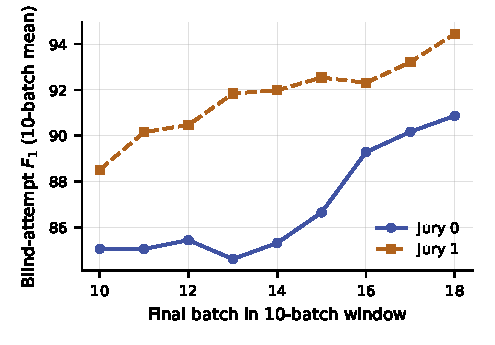
\includegraphics[width=\columnwidth]{figs/learning_trend.pdf}
\caption{Blind-attempt $F_1$ of the two NoPnx-PA juries during training, averaged over a
moving window of 10 batches (50 documents), in curriculum order. Each attempt is scored
before the gold for its batch is revealed and no document is seen twice, so the curve
reflects performance on unseen documents as the policy files grow. The juries train on
disjoint halves of the corpus. NoPnx-PA is the track whose full training run is banked
end to end; the other tracks' juries were trained across several sessions and their
attempts are not recoverable in curriculum order.}
\label{fig:curve}
\end{figure}

\end{document}
